\documentclass[conference]{IEEEtran}
\IEEEoverridecommandlockouts

\usepackage{cite}
\usepackage{amsmath,amssymb,amsfonts}
\usepackage{graphicx}
\usepackage{booktabs}
\usepackage{multirow}
\usepackage{xcolor}
\usepackage{tikz}
\usetikzlibrary{positioning,arrows.meta,fit}
\usepackage{pgfplots}
\pgfplotsset{compat=1.17}
\usepackage{url}

% Forces a new row of author blocks (IEEEtran has no built-in command).
\makeatletter
\newcommand{\linebreakand}{%
  \end{@IEEEauthorhalign}
  \hfill\mbox{}\par
  \mbox{}\hfill\begin{@IEEEauthorhalign}
}
\makeatother

\begin{document}

\title{Spatial--Frequency Fusion and Temporal Transformers for Deepfake Video Detection: A Leakage-Aware Evaluation}

% Three authors on the first row, two centred on the second.
\author{
\IEEEauthorblockN{1\textsuperscript{st} Ayush Tiwari}
\IEEEauthorblockA{\textit{KIET Deemed to be University}\\
Delhi-NCR, Ghaziabad, India}
\and
\IEEEauthorblockN{2\textsuperscript{nd} Atharv Shukla}
\IEEEauthorblockA{\textit{KIET Deemed to be University}\\
Delhi-NCR, Ghaziabad, India}
\and
\IEEEauthorblockN{3\textsuperscript{rd} Ayushman Patel}
\IEEEauthorblockA{\textit{KIET Deemed to be University}\\
Delhi-NCR, Ghaziabad, India}
\linebreakand
\IEEEauthorblockN{4\textsuperscript{th} Bhanupratap Chaurasia}
\IEEEauthorblockA{\textit{KIET Deemed to be University}\\
Delhi-NCR, Ghaziabad, India}
\and
\IEEEauthorblockN{5\textsuperscript{th} Mayank Lakhotia}
\IEEEauthorblockA{\textit{KIET Deemed to be University}\\
Delhi-NCR, Ghaziabad, India}
}

\maketitle

\begin{abstract}
Hybrid deepfake detectors increasingly combine pixel-domain appearance,
frequency-domain artifacts and temporal cues, but the contribution of each
component is rarely isolated under a protocol that prevents leakage and
accounts for small test sets. We build a video-level detector in which an
ImageNet-pretrained ResNet18 encodes each face crop, a lightweight
convolutional network encodes its log-magnitude 2D Fourier spectrum, and a
Transformer encoder models the sequence of fused per-frame embeddings. On the
400-video DeepFake Detection Challenge (DFDC) training sample, with splits that
keep every fake with its source video and thresholds chosen on validation data
only, we compare the hybrid with an ablation that replaces the Transformer by
temporal averaging and with a frame-level ResNet18 baseline over three random
seeds. Both frequency-augmented models reach a higher F1 than the baseline on
every seed (mean 0.848 and 0.792 against 0.642), but test ROC-AUC is similar
(0.715, 0.745 and 0.700), the Transformer gives no consistent gain over
averaging, and paired DeLong tests find no significant difference in any of
the nine within-seed comparisons ($p \geq 0.067$). Because test splits are 80\%
fake, a detector that labels every video FAKE scores higher accuracy and F1
than every model, so threshold-free metrics are essential at this scale. We
release the complete CPU-trainable pipeline and argue that claims of
improvement from hybrid designs need larger test sets and paired statistical
tests.
\end{abstract}

\begin{IEEEkeywords}
Deepfake detection, video forensics, frequency analysis, Fourier transform,
Transformer encoder, temporal modeling, ResNet18, DFDC
\end{IEEEkeywords}

%=====================================================================
\section{Introduction}
%=====================================================================

It no longer takes a studio or a specialist to swap or re-animate a face in a
video; a consumer GPU and a few hours of tutorials are enough
\cite{tolosana2020survey,mirsky2021survey}. The resulting ``deepfakes'' have
already been used for harassment, fraud and political misinformation, and
there is far more of this material than any team of human reviewers could
check. Automatic detection has become a practical necessity.

The first learned detectors treated the task as ordinary image classification:
crop the face, run a convolutional network, read off a real/fake score
\cite{afchar2018mesonet,rossler2019faceforensics}. That recipe works well when
the training and test fakes come from the same manipulation method, but it
throws away two things. One is the frequency domain. The upsampling layers
inside generators leave regular patterns in the spectrum that are nearly
invisible in pixel space
\cite{durall2020watch,frank2020leveraging,qian2020thinking}. The other is
time. A fake is assembled largely frame by frame, so identity, lighting and
expression can flicker in ways that no single frame will show
\cite{guera2018deepfake,zheng2021exploring}.

Recent detectors combine these cues, fusing RGB and frequency streams
\cite{luo2021highfreq,gu2022pel,wang2023sfdg} or modeling time with 3D
networks and video Transformers \cite{wang2023altfreezing,zhao2023istvt}.
Such systems are usually evaluated as a whole, which leaves open how much each
component contributes. We ask that question directly. Our detector
(Fig.~\ref{fig:arch}) runs each sampled face through a spatial and a spectral
branch, fuses the two embeddings for that frame, and passes the ordered
sequence through a Transformer encoder \cite{vaswani2017attention} before
making one decision for the whole video. Comparing it with an ablation without
the Transformer and with a frame-level ResNet18 \cite{he2016deep} isolates the
frequency branch and the temporal module in turn.

The contributions of this work are:
\begin{itemize}
\item A leakage-aware evaluation protocol for small video datasets: splits
  grouped by source video, decision thresholds chosen on validation data
  only, bootstrap confidence intervals, and paired DeLong tests
  \cite{delong1988auc} between models scored on the same videos.
\item A controlled three-way comparison on the DFDC training sample, over
  three seeds, that separates the effect of the frequency branch from that of
  the temporal Transformer.
\item Empirical findings: the frequency branch raises F1 at the operating
  point, but neither it nor the Transformer yields a statistically
  significant ROC-AUC gain, and under the 80\% fake class balance a trivial
  all-FAKE detector beats every model on accuracy and F1.
\item An open, CPU-trainable implementation covering frame sampling, face
  cropping, training, evaluation, single-video inference and a web demo.
\end{itemize}

\begin{figure*}[t]
\centering
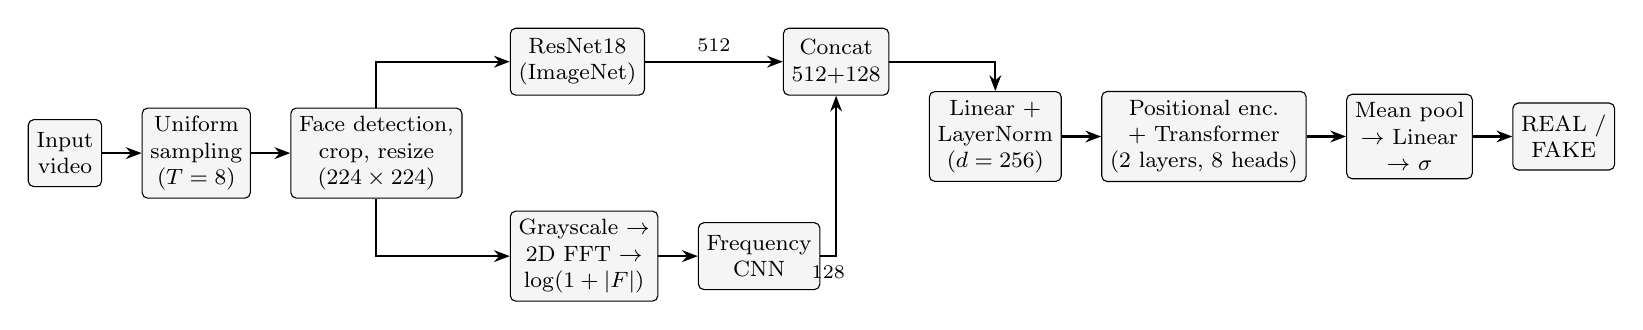
\begin{tikzpicture}[
  node distance=0.35cm and 0.5cm,
  box/.style={draw, rounded corners=2pt, align=center, font=\footnotesize,
              minimum height=0.85cm, inner sep=3pt, fill=gray!8},
  arr/.style={-{Stealth[length=2mm]}, thick}]
\node[box] (video) {Input\\video};
\node[box, right=of video] (sample) {Uniform\\sampling\\($T=8$)};
\node[box, right=of sample] (face) {Face detection,\\crop, resize\\($224\times224$)};
\node[box, above right=0.15cm and 0.6cm of face] (res) {ResNet18\\(ImageNet)};
\node[box, below right=0.15cm and 0.6cm of face] (fft) {Grayscale $\rightarrow$\\2D FFT $\rightarrow$\\$\log(1+|F|)$};
\node[box, right=of fft] (fcnn) {Frequency\\CNN};
\node[box, right=1.75cm of res] (cat) {Concat\\$512{+}128$};
\node[box, right=of cat, yshift=-0.95cm] (proj) {Linear +\\LayerNorm\\($d=256$)};
\node[box, right=of proj] (tf) {Positional enc.\\+ Transformer\\(2 layers, 8 heads)};
\node[box, right=of tf] (head) {Mean pool\\$\rightarrow$ Linear\\$\rightarrow$ $\sigma$};
\node[box, right=of head] (out) {REAL /\\FAKE};
\draw[arr] (video) -- (sample);
\draw[arr] (sample) -- (face);
\draw[arr] (face) |- (res);
\draw[arr] (face) |- (fft);
\draw[arr] (fft) -- (fcnn);
\draw[arr] (res) -- node[above, font=\scriptsize]{512} (cat);
\draw[arr] (fcnn) -| node[pos=0.25, below, font=\scriptsize]{128} (cat);
\draw[arr] (cat) -| (proj);
\draw[arr] (proj) -- (tf);
\draw[arr] (tf) -- (head);
\draw[arr] (head) -- (out);
\end{tikzpicture}
\caption{Proposed architecture. Both branches run on every sampled face crop
with shared weights; the fused per-frame embeddings form a sequence of length
$T$ that the Transformer encoder models before a single video-level decision.}
\label{fig:arch}
\end{figure*}

%=====================================================================
\section{Background and Related Work}
\label{sec:related}
%=====================================================================

Detection methods have moved through roughly four phases, and our design
borrows from the last three.

\textit{Hand-crafted cues.} The earliest work relied on physical or semantic
cues: abnormal eye blinking \cite{li2018ictu}, head poses inconsistent with
the face \cite{yang2019headpose}, and visual artifacts such as implausible eye
colour, missing tooth detail or mismatched reflections \cite{matern2019visual}.
Each cue depends on a specific flaw, and later synthesis tools tend to fix
exactly that flaw.

\textit{Spatial detectors.} Learned features took over next. MesoNet
\cite{afchar2018mesonet} used a deliberately shallow network tuned to
mesoscopic image properties, and the FaceForensics++ benchmark
\cite{rossler2019faceforensics} showed that a general-purpose classifier such
as XceptionNet \cite{chollet2017xception}, trained on face crops, was already
a hard baseline to beat. Fine-tuned ImageNet backbones
\cite{he2016deep,deng2009imagenet} remain strong on in-distribution data but
degrade on unseen manipulation methods \cite{tolosana2020survey,mirsky2021survey}.
Much recent work therefore targets generalisation: training on self-blended
real faces \cite{shiohara2022sbi}, learning the distribution of real faces by
reconstruction \cite{cao2022recce}, separating method-specific from common
forgery features \cite{yan2023ucf}, or attending to localised artifacts
\cite{nguyen2024laanet}. DeepfakeBench \cite{yan2023deepfakebench} showed how
strongly reported numbers depend on preprocessing and protocol, and
standardised both across many detectors.

\textit{Frequency-domain detectors.} Generated images carry characteristic
artifacts in their Fourier spectra, a side effect of upsampling
\cite{durall2020watch,frank2020leveraging}, and a classifier trained on one
generator can transfer surprisingly well to others \cite{wang2020cnn}.
F\textsuperscript{3}-Net \cite{qian2020thinking} built frequency-aware
decomposition and local frequency statistics into a two-stream face forgery
detector. Later work fused RGB with high-frequency residuals through
cross-modality attention \cite{luo2021highfreq}, progressively enhanced and
fused RGB and fine-grained frequency streams \cite{gu2022pel}, reasoned over
spatial and frequency features with dynamic graphs \cite{wang2023sfdg}, and
learned directly in the FFT amplitude and phase domain with a lightweight
network \cite{tan2024freqnet}.

\textit{Temporal detectors.} The most recent phase treats a video as a
sequence rather than a bag of frames. Recurrent networks over per-frame CNN
features \cite{guera2018deepfake}, temporal-coherence models
\cite{zheng2021exploring} and analyses of mouth movement
\cite{haliassos2021lips} exploit the fact that fakes are synthesised largely
one frame at a time. Transformers \cite{vaswani2017attention} have become a
standard tool for sequence modeling in vision \cite{dosovitskiy2021image}, and
video Transformers \cite{bertasius2021space,arnab2021vivit} model space and
time jointly at a high training cost. In deepfake detection, CNN features have
been combined with Vision Transformers and evaluated on DFDC
\cite{coccomini2022effvit}, spatial and temporal self-attention have been
factorised for interpretability \cite{zhao2023istvt}, spatial and temporal
weights have been trained alternately so that neither dominates
\cite{wang2023altfreezing}, frames have been tiled into thumbnails so a 2D
backbone sees temporal change \cite{xu2023tall}, the temporal flow of style
latents has been used as a cue \cite{choi2024stylelatent}, and frequency
clues have been extracted along both spatial and temporal axes
\cite{wang2023stfclue}.

\textit{Datasets.} FaceForensics++ \cite{rossler2019faceforensics} contains
1{,}000 YouTube videos manipulated by four methods at several compression
levels. Celeb-DF \cite{li2020celeb} offers higher-quality fakes and is the
usual choice for testing whether a detector generalises across datasets. The
DeepFake Detection Challenge (DFDC) \cite{dolhansky2019preview,dolhansky2020dfdc}
released videos of paid, consenting actors and links each fake to its source
video, which is what makes a leakage-free split possible.

\textit{Positioning of this work.} The hybrid systems above are trained on
large datasets with GPUs and evaluated as complete models, typically against
other published detectors. Our work is complementary: rather than proposing a
stronger detector, we take a compact spatial--frequency--temporal design and
measure what each component adds under a protocol built for small data,
with source-grouped splits, validation-only thresholds, confidence intervals
and paired significance tests.

%=====================================================================
\section{Dataset and Preprocessing}
%=====================================================================

\subsection{Dataset}
We worked with the training sample of the DFDC \cite{dolhansky2020dfdc}: 400
videos of roughly 10\,s each at $1920\times1080$, of which 77 are real and 323
are fake. The accompanying \texttt{metadata.json} names the original video
that each fake was made from. We were unable to complete the official download
for our account before the deadline, so the files came from a public Kaggle
re-upload containing the same 400 videos and a \texttt{metadata.json} in the
official format. We return to this in the Discussion. The data were used only
for this research and have not been redistributed.

\subsection{Leakage-aware split}
Every video was assigned to the source group of its original, which gave 244
groups. We then shuffled the groups, not the videos, with a fixed seed and
divided them 70/15/15 within each class, counting a group as real if it
contains a real video. A check in the code refuses any split in which a video
or group turns up in more than one partition. Because whole groups are
assigned, the number of videos per partition varies with the seed.
Table~\ref{tab:split} shows the three splits used in this paper.

\begin{table}[t]
\caption{Grouped Splits of the DFDC Sample (Videos, Real/Fake)}
\label{tab:split}
\centering
\footnotesize
\begin{tabular}{lccc}
\toprule
\textbf{Split} & \textbf{Seed 42} & \textbf{Seed 7} & \textbf{Seed 123} \\
\midrule
Train & 294 (54/240) & 277 (54/223) & 297 (54/243) \\
Validation & 54 (12/42) & 54 (12/42) & 55 (12/43) \\
Test & 52 (11/41) & 69 (11/58) & 48 (11/37) \\
\bottomrule
\end{tabular}
\end{table}

\subsection{Frame sampling and face cropping}
From each video we take $T=8$ frames at evenly spaced indices computed from
that video's own length, so the same video always yields the same frames.
Faces are located with OpenCV's Haar cascade \cite{viola2001rapid}, run on a
copy of the frame downscaled to at most 640\,px to keep it fast. We take the
largest detection, pad it by 25\%, make it square, clamp it to the frame and
resize it to $224\times224$ (Fig.~\ref{fig:seq}). If a frame has no detection
we reuse the box from the nearest earlier frame, failing that the nearest
later one, and as a last resort fall back to a centre crop, so a video always
produces exactly $T$ crops. The cascade found a face in 2{,}339 of the 3{,}176
frames it examined (73.6\%); 32 videos had no detection at all and ended up as
centre crops. Crops are cached as 8-bit arrays so that training does not have
to decode video over and over. During training we apply light augmentation
(horizontal flip, rotation within $\pm5^\circ$, mild brightness and contrast
jitter) identically to every frame of a sequence and before the Fourier
transform, so both branches always see the same image.

\begin{figure}[t]
\centering
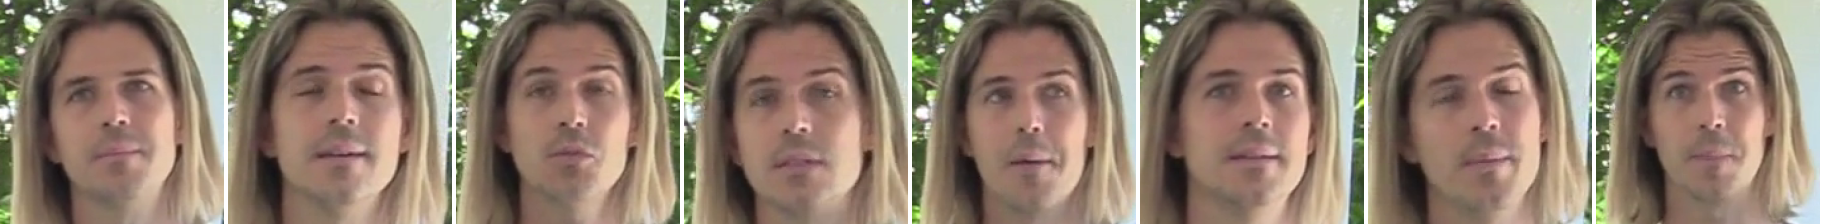
\includegraphics[width=\columnwidth]{figures/frame_sequence.png}
\caption{The eight face crops sampled from one real test video.}
\label{fig:seq}
\end{figure}

%=====================================================================
\section{Proposed Methodology}
%=====================================================================

We write a video as its face crops $x_1,\dots,x_T$, each
$x_t\in\mathbb{R}^{3\times224\times224}$ normalised with ImageNet statistics.

\subsection{Spatial branch}
An ImageNet-pretrained ResNet18 \cite{he2016deep} with its classification
layer removed maps each crop to a 512-dimensional embedding
$s_t = \phi_{\mathrm{RGB}}(x_t)$. We fine-tune all of its layers rather than
freezing the backbone.

\subsection{Frequency branch}
Each crop is first de-normalised back to $[0,1]$, so that the spectrum
reflects real pixel values rather than standardised ones, and converted to
grayscale $g_t$. Its 2D discrete Fourier transform is
\begin{equation}
F_t(u,v)=\sum_{x=0}^{H-1}\sum_{y=0}^{W-1} g_t(x,y)\,
e^{-j2\pi\left(\frac{ux}{H}+\frac{vy}{W}\right)}.
\end{equation}
We shift the zero frequency to the centre and take the log-magnitude
$M_t=\log\!\left(1+|F_t|\right)$, which tames the spectrum's wide dynamic
range and avoids numerical trouble at zero, then min--max normalise each
image to $[0,1]$. Fig.~\ref{fig:fft} shows what the branch sees. A small CNN
of four blocks (3$\times$3 convolution, batch normalisation, ReLU, 2$\times$2
max pooling, with 16, 32, 64 and 128 channels), followed by global average
pooling and a linear layer, turns $M_t$ into a 128-dimensional embedding
$f_t$. The whole branch has about 0.11\,M parameters. The transform itself
runs inside the model on the same device as everything else, so there is no
second preprocessing cache to maintain. We do not assume that the spectrum
identifies fakes on its own. It is simply another view of the same crop, from
which the network may or may not pick up useful cues.

\begin{figure}[t]
\centering
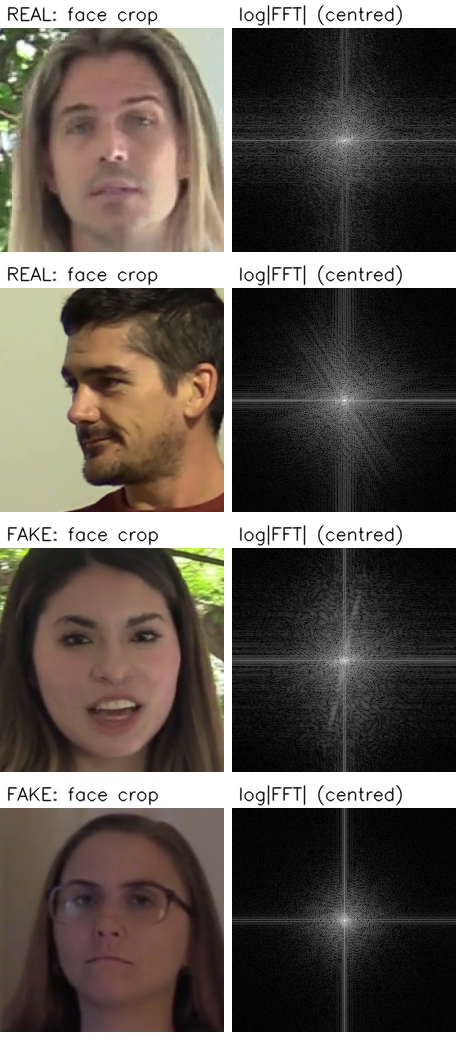
\includegraphics[width=0.78\columnwidth]{figures/fft_examples.png}
\caption{Face crops from test videos (left) and the normalised log-magnitude
spectra given to the frequency branch (right).}
\label{fig:fft}
\end{figure}

\subsection{Per-frame fusion}
The two embeddings are concatenated and projected to a common width
$d=256$:
\begin{equation}
z_t=\mathrm{LayerNorm}\!\left(W\,[s_t;f_t]+b\right),\quad
W\in\mathbb{R}^{256\times640}.
\end{equation}
The layer normalisation is there because the two branches produce activations
on quite different scales, and the next stage is easier to train when that
difference is removed. Both branches share weights across the $T$ frames.

\subsection{Temporal Transformer}
We add fixed sinusoidal positional encodings \cite{vaswani2017attention} to
$z_1,\dots,z_T$ so the model knows the frame order, then pass the sequence
through a two-layer Transformer encoder with 8 heads, a feed-forward width of
1024, pre-norm and dropout 0.1. The Transformer here is a sequence model over
eight numeric vectors; there is no tokenizer and no language objective
involved.

\subsection{Classification and loss}
The encoder outputs are averaged over time and a linear layer maps the result
to a single logit $\ell$; $p=\sigma(\ell)$ is the model's estimate that the
video is fake. The training splits hold 4.1 to 4.5 fakes for every real video,
so we weight the positive class in the binary cross-entropy by
$w=N_{\mathrm{real}}/N_{\mathrm{fake}}$, computed on the training split
($w=0.225$, $0.242$ and $0.222$ for seeds 42, 7 and 123):
\begin{equation}
\mathcal{L}=-\left[w\,y\log p+(1-y)\log(1-p)\right].
\end{equation}
Without the weighting a model can drive the loss down simply by calling
everything FAKE. Validation and test losses are reported unweighted.

\subsection{Baseline and ablation}
The baseline runs the same pretrained ResNet18 on each frame, a shared linear
head gives one logit per frame, and the video logit is the mean of the $T$
frame logits. There is no frequency branch, no fusion and no Transformer.
To isolate the temporal module we also train an ablation that keeps both
branches and the fusion step but drops the positional encoding and the
Transformer, so the fused embeddings $z_t$ are simply averaged over time
before the linear head. Everything else, the data, the split, the loss and
the optimizer, is identical across the three models, so differences between
them should come down to the architecture.

\subsection{Metrics, thresholds and statistical tests}
FAKE is the positive class. We report accuracy, precision, recall and F1 at a
decision threshold, the confusion matrix, and the threshold-free area under
the ROC curve (ROC-AUC) \cite{fawcett2006introduction}, for which 0.5 is chance
level. Thresholds are either the default 0.5 or the value that maximises
Youden's $J=\mathrm{TPR}-\mathrm{FPR}$ \cite{youden1950index} on the
\emph{validation} split, which is then applied to the test split unchanged; the
test split is never used to pick a threshold or a checkpoint. For each test
result we compute a 95\% percentile bootstrap interval for ROC-AUC and F1 from
2{,}000 resamples of the test videos, drawn separately within the real and the
fake videos so that every resample keeps the split's class counts. Because
models trained under the same seed are scored on the same test videos, we
compare their ROC-AUCs with the paired DeLong test \cite{delong1988auc}, which
accounts for the correlation between the two sets of scores.

%=====================================================================
\section{Implementation}
%=====================================================================

The system is written in Python with PyTorch \cite{paszke2019pytorch},
torchvision, OpenCV and scikit-learn \cite{pedregosa2011scikit}, as small
modules for video reading, face extraction, dataset and splits, models,
training, evaluation, inference and the user interface, with automated checks
for every stage. Table~\ref{tab:config} lists the training settings. The best
checkpoint is picked by validation ROC-AUC and saved together with its full
configuration, so inference rebuilds exactly the model that was trained. All
experiments ran on a laptop with an Intel Core i7-7500U CPU (2 cores,
4 threads), 32\,GB of RAM and no GPU; one epoch of the hybrid model took
8--10\,min when the machine was otherwise idle.

\textit{Inference cost.} On the same CPU, one forward pass over an 8-frame
clip (median of 20 runs) takes 443\,ms for the baseline, 643\,ms without the
Transformer and 648\,ms for the full hybrid. The frequency branch is
therefore the main added cost, while the Transformer adds 1.6\,M parameters
but little time. The full single-video pipeline, including decoding a
1080p video and face detection, takes 6.3--7.1\,s, so preprocessing rather
than the network dominates inference time.

\begin{table}[t]
\caption{Model and Training Configuration}
\label{tab:config}
\centering
\footnotesize
\begin{tabular}{ll}
\toprule
\textbf{Setting} & \textbf{Value} \\
\midrule
Frames per video / crop size & 8 / $224\times224$ \\
Spatial / frequency embedding & 512 / 128 \\
Fused width $d$ & 256 \\
Transformer & 2 layers, 8 heads, FFN 1024 \\
Optimizer & AdamW \cite{loshchilov2019decoupled}, lr $10^{-4}$, wd $10^{-4}$ \\
Batch size / epochs & 2 / 5 \\
Model selection & best validation ROC-AUC \\
Seeds & 42, 7, 123 \\
Parameters & hybrid 13.03\,M, no Transformer 11.46\,M, \\
 & baseline 11.18\,M \\
Hardware & Intel Core i7-7500U CPU, no GPU \\
\bottomrule
\end{tabular}
\end{table}

A command-line tool takes a video file and a checkpoint and prints REAL or
FAKE, the model's fake probability, the number of frames used and how many of
them contained a detected face. A minimal Streamlit web interface wraps the
same function: the user uploads a video, previews it, and gets back the
prediction alongside one of the face crops the model actually saw. The
probability shown is the raw sigmoid output and has not been calibrated. The
code, configurations and per-video test predictions are available at
\url{https://github.com/Ayush29bit/DeepFake-Detection}.

%=====================================================================
\section{Results and Evaluation}
%=====================================================================

\subsection{Experimental setup}
Each of the three models was trained for five epochs under three seeds (42, 7
and 123). The seed fixes the grouped split and the weight initialisation, so
the three models trained under one seed saw exactly the same split
(Table~\ref{tab:split}); the random draws of the training augmentation are not
seeded. For every run the checkpoint with the best validation ROC-AUC was
evaluated once on that seed's test split. Since the test split changes with
the seed, models are compared within a seed, and the means and standard
deviations below summarise the three seeds.

\subsection{Results}
Table~\ref{tab:results} gives the mean and standard deviation over the three
seeds, Table~\ref{tab:seeds} the per-seed ROC-AUC and F1 with their
bootstrap intervals, and Table~\ref{tab:delong} the paired DeLong tests.
Every test split is about 80\% fake, so a trivial
detector that labels every video FAKE would reach an accuracy of 0.800 and an
F1 of 0.889 on average, with ROC-AUC 0.5. We list it as a reference point.
Fig.~\ref{fig:roc} shows the ROC curves, Fig.~\ref{fig:cm} the confusion
matrices at the validation-chosen threshold and Fig.~\ref{fig:loss} the loss
curves for seed 42.

\begin{table*}[t]
\caption{Test Results, Mean $\pm$ Standard Deviation over Seeds 42, 7 and 123}
\label{tab:results}
\centering
\footnotesize
\setlength{\tabcolsep}{4pt}
\begin{tabular}{llccccc}
\toprule
\textbf{Model} & \textbf{Threshold} & \textbf{Accuracy} & \textbf{Precision} &
\textbf{Recall} & \textbf{F1} & \textbf{ROC-AUC} \\
\midrule
\multirow{2}{*}{ResNet18 baseline} & 0.5 & $0.444\pm0.109$ & $0.869\pm0.028$ & $0.359\pm0.164$ & $0.492\pm0.179$ & \multirow{2}{*}{$0.700\pm0.057$} \\
 & validation & $0.553\pm0.108$ & $0.870\pm0.032$ & $0.526\pm0.178$ & $0.642\pm0.119$ & \\
\midrule
\multirow{2}{*}{Hybrid, no Transformer} & 0.5 & $0.679\pm0.185$ & $0.913\pm0.081$ & $0.672\pm0.292$ & $0.742\pm0.195$ & \multirow{2}{*}{$0.745\pm0.073$} \\
 & validation & $0.696\pm0.076$ & $0.873\pm0.035$ & $0.732\pm0.112$ & $0.792\pm0.061$ & \\
\midrule
\multirow{2}{*}{Hybrid (proposed)} & 0.5 & $0.704\pm0.010$ & $0.875\pm0.020$ & $0.734\pm0.006$ & $0.798\pm0.012$ & \multirow{2}{*}{$0.715\pm0.107$} \\
 & validation & $0.770\pm0.087$ & $0.880\pm0.048$ & $0.822\pm0.102$ & $0.848\pm0.065$ & \\
\midrule
Always FAKE (reference) & -- & $0.800\pm0.036$ & $0.800\pm0.036$ & $1.000$ & $0.889\pm0.022$ & $0.500$ \\
\bottomrule
\end{tabular}
\end{table*}

\begin{table*}[t]
\caption{Per-Seed Test Results with 95\% Bootstrap Intervals (F1 and Confusion Matrix at the Validation-Chosen Threshold)}
\label{tab:seeds}
\centering
\footnotesize
\setlength{\tabcolsep}{4pt}
\begin{tabular}{lcccccc}
\toprule
\textbf{Model} & \textbf{Seed} & \textbf{Test videos} & \textbf{Threshold} &
\textbf{ROC-AUC [95\% CI]} & \textbf{F1 [95\% CI]} & \textbf{TN/FP/FN/TP} \\
\midrule
\multirow{3}{*}{ResNet18 baseline} & 42 & 52 & 0.099 & 0.665 [0.455, 0.851] & 0.779 [0.676, 0.867] & 5/6/11/30 \\
 & 7 & 69 & 0.598 & 0.669 [0.473, 0.862] & 0.565 [0.441, 0.681] & 8/3/34/24 \\
 & 123 & 48 & 0.535 & 0.767 [0.590, 0.916] & 0.582 [0.417, 0.712] & 9/2/21/16 \\
\midrule
\multirow{3}{*}{Hybrid, no Transformer} & 42 & 52 & 0.154 & 0.827 [0.698, 0.933] & 0.831 [0.740, 0.909] & 7/4/9/32 \\
 & 7 & 69 & 0.618 & 0.688 [0.481, 0.868] & 0.722 [0.622, 0.808] & 7/4/23/35 \\
 & 123 & 48 & 0.446 & 0.720 [0.555, 0.877] & 0.822 [0.735, 0.897] & 5/6/7/30 \\
\midrule
\multirow{3}{*}{Hybrid (proposed)} & 42 & 52 & 0.442 & 0.612 [0.386, 0.831] & 0.815 [0.730, 0.884] & 4/7/8/33 \\
 & 7 & 69 & 0.396 & 0.708 [0.505, 0.887] & 0.923 [0.877, 0.959] & 6/5/4/54 \\
 & 123 & 48 & 0.562 & 0.826 [0.693, 0.941] & 0.806 [0.698, 0.896] & 8/3/10/27 \\
\bottomrule
\end{tabular}
\end{table*}

\begin{table}[t]
\caption{Paired DeLong Tests of Test ROC-AUC Within Each Seed ($\Delta$ = first model minus second; two-sided $p$)}
\label{tab:delong}
\centering
\footnotesize
\setlength{\tabcolsep}{4pt}
\begin{tabular}{lcccccc}
\toprule
 & \multicolumn{2}{c}{\textbf{Hybrid vs. base}} & \multicolumn{2}{c}{\textbf{No-Tr. vs. base}} & \multicolumn{2}{c}{\textbf{Hybrid vs. No-Tr.}} \\
\textbf{Seed} & $\Delta$ & $p$ & $\Delta$ & $p$ & $\Delta$ & $p$ \\
\midrule
42 & $-0.053$ & 0.736 & $+0.162$ & 0.067 & $-0.215$ & 0.067 \\
7 & $+0.039$ & 0.611 & $+0.019$ & 0.879 & $+0.020$ & 0.789 \\
123 & $+0.059$ & 0.250 & $-0.047$ & 0.673 & $+0.106$ & 0.169 \\
\bottomrule
\end{tabular}
\end{table}

\begin{figure*}[t]
\centering
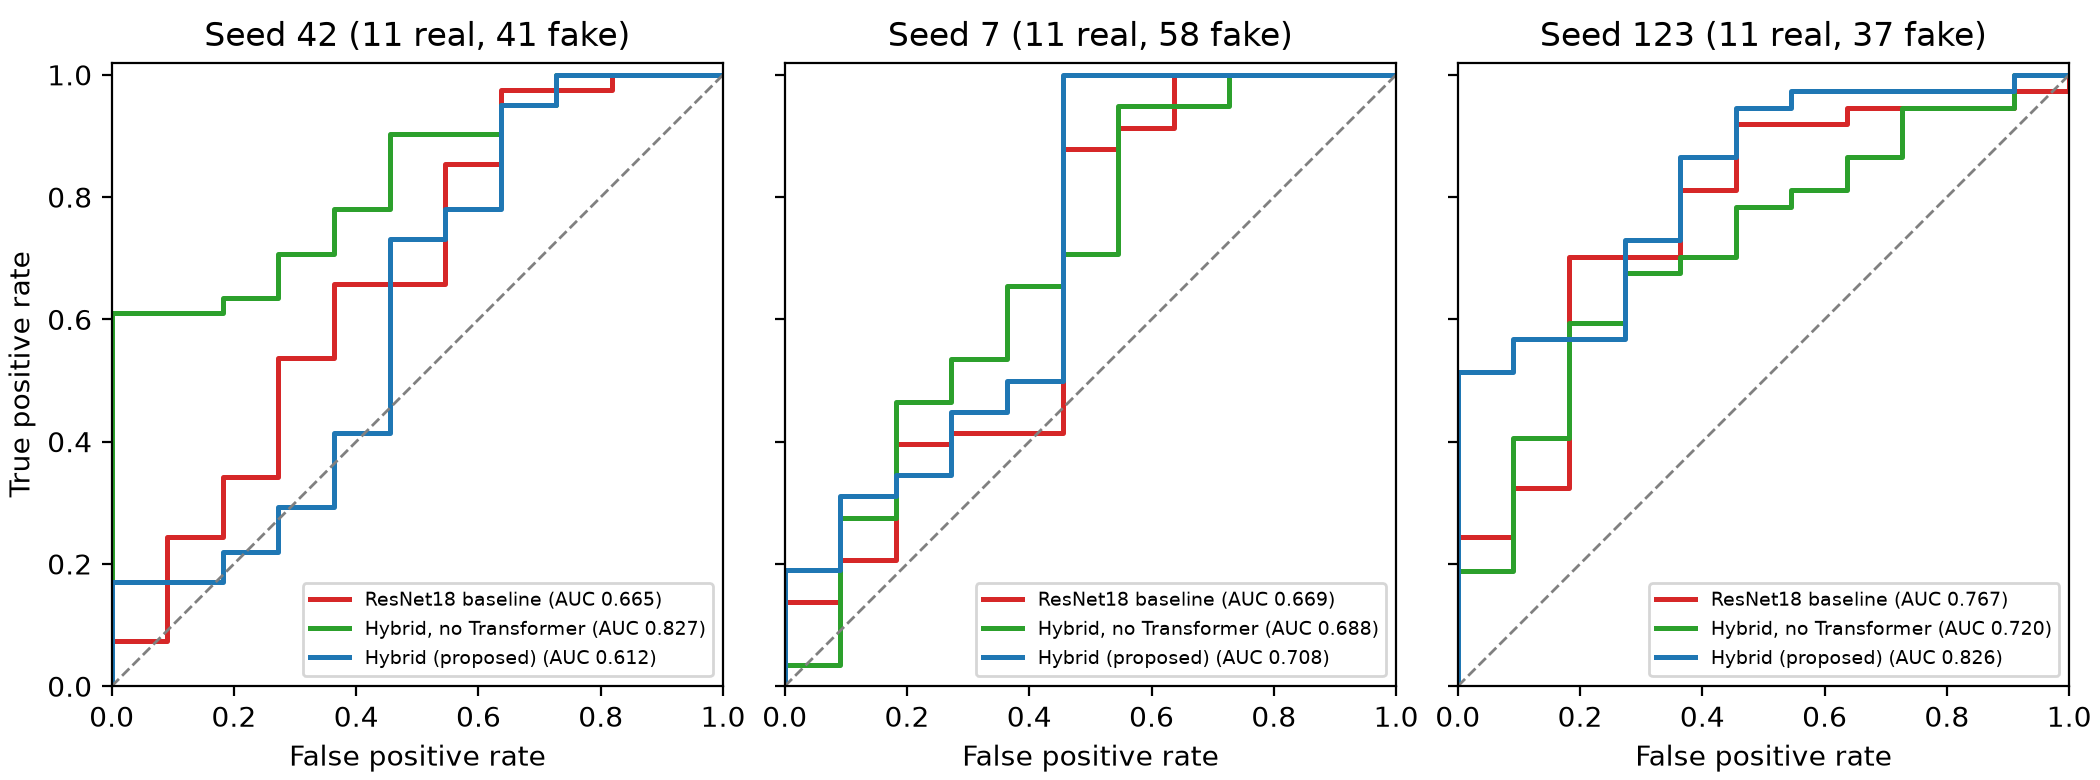
\includegraphics[width=\textwidth]{figures/roc_curves.png}
\caption{Test ROC curves for each seed. Each panel uses that seed's own test
split; the dashed diagonal is chance level.}
\label{fig:roc}
\end{figure*}

\begin{figure*}[t]
\centering
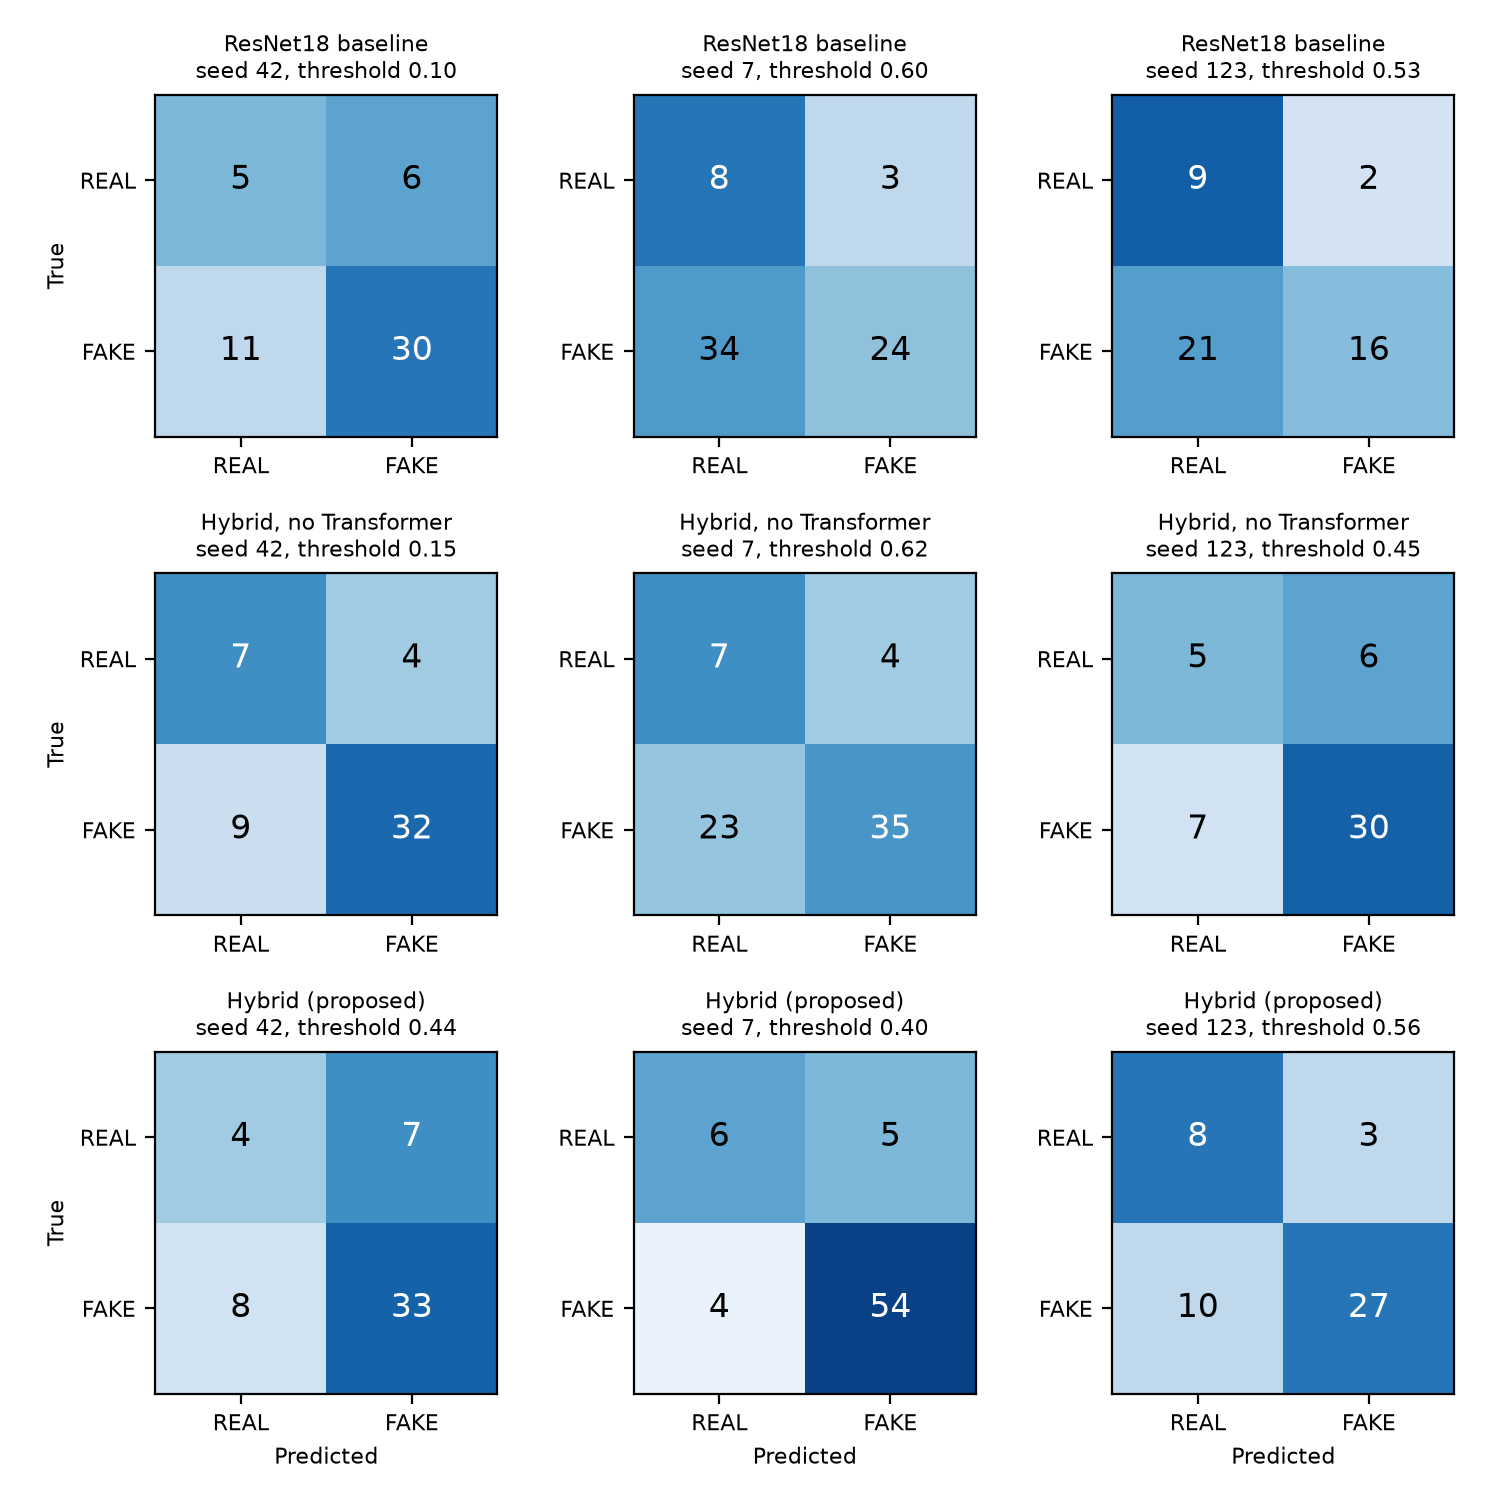
\includegraphics[width=0.62\textwidth]{figures/confusion_matrices.png}
\caption{Test confusion matrices at the validation-chosen threshold (rows: true
class, columns: predicted class). Shading shows the share of each true class.}
\label{fig:cm}
\end{figure*}

\begin{figure}[t]
\centering
\begin{tikzpicture}
\begin{axis}[width=\columnwidth, height=4.6cm, xlabel={Epoch},
  ylabel={Loss}, xtick={1,2,3,4,5}, legend style={font=\scriptsize,
  at={(0.98,0.98)}, anchor=north east}, tick label style={font=\scriptsize},
  label style={font=\footnotesize}]
\addplot[blue, mark=*] table[x=epoch, y=train_loss, col sep=comma] {data/dfdc_hybrid.csv};
\addplot[blue, dashed, mark=o] table[x=epoch, y=val_loss, col sep=comma] {data/dfdc_hybrid.csv};
\addplot[red, mark=square*] table[x=epoch, y=train_loss, col sep=comma] {data/dfdc_baseline_5ep.csv};
\addplot[red, dashed, mark=square] table[x=epoch, y=val_loss, col sep=comma] {data/dfdc_baseline_5ep.csv};
\legend{Hybrid train, Hybrid val, Baseline train, Baseline val}
\end{axis}
\end{tikzpicture}
\caption{Training (class-weighted) and validation (unweighted) loss, seed 42.}
\label{fig:loss}
\end{figure}

\subsection{Analysis}
Reading Tables~\ref{tab:results} and~\ref{tab:seeds} together with
Figs.~\ref{fig:roc} and~\ref{fig:cm}, four things stand out.

First, the frequency branch appears to help at the operating point. Both
models that include it reached a higher F1 than the baseline on every seed at
the validation-chosen threshold (mean 0.848 and 0.792 against 0.642). On
ROC-AUC, which does not depend on the threshold, the gap is much smaller
(0.715 and 0.745 against 0.700), and each hybrid variant beat the baseline on
only two of the three seeds.

Second, the Transformer gave no consistent gain over simple averaging. The full
hybrid had the higher ROC-AUC on seeds 7 and 123 but by far the lower one on
seed 42 (0.612 against 0.827), and the higher F1 on seed 7 only. On seed 42
the variant without the Transformer had the best ROC-AUC, accuracy and F1 of
the three models, while the full hybrid had the worst ROC-AUC. The one property in which the full
hybrid stood out was stability at the default threshold: its F1 at 0.5 varied
by only $\pm0.012$ across seeds, against $\pm0.179$ for the baseline and
$\pm0.195$ for the ablation, and its validation-chosen thresholds stayed
between 0.40 and 0.56, while the other two models' ranged from 0.10 to 0.62.

Third, none of these differences is statistically significant. In the paired
DeLong tests (Table~\ref{tab:delong}) no comparison reaches $p<0.05$; the
closest are the seed-42 gaps between the ablation and the other two models
($p=0.067$), and neither gap keeps its size or direction on the other seeds. With 11
real videos in each test split, a single misclassified real video moves the
false positive rate by about nine percentage points, the 95\% intervals for
ROC-AUC are between 0.24 and 0.45 wide, and the seed-42 interval of the full
hybrid, [0.386, 0.831], even includes chance level.

Fourth, accuracy and F1 flatter every model here. Because about 80\% of the
test videos are fake, labelling everything FAKE scores higher than every
trained model on mean accuracy and mean F1 (Table~\ref{tab:results}); a
trained model beat it only on seed 7. These two metrics mainly reflect where
the threshold sits, and ROC-AUC, together with the full confusion matrices, is
the fairer basis for comparison. Fig.~\ref{fig:cm} also shows that the models
fail in different ways: at its validation-chosen threshold the baseline missed
21 to 34 fakes on seeds 7 and 123, while the full hybrid on seed 42 flagged 7
of the 11 real videos as fake.

The validation and test results also disagreed noticeably. The full hybrid
reached a validation ROC-AUC of 0.861, 0.788 and 0.868 on the three seeds but
0.612, 0.708 and 0.826 on test, and the baseline's best seed-42 checkpoint
came from epoch 1, after which its validation loss became erratic
(Fig.~\ref{fig:loss}). With 54 or 55 validation videos, model selection itself
is noisy, which is a further reason not to read much into any single run.

%=====================================================================
\section{Discussion and Challenges}
%=====================================================================

\textit{Data scale.} The size of the test splits is the biggest limitation of
this study. Three seeds give a sense of the run-to-run variation, but with 11
real videos per test split the confidence intervals are too wide to rank the
three models. Larger test sets, not more seeds on the same 400 videos, are
what would settle the question.

\textit{Face detection.} The Haar cascade missed faces in 26\% of frames and
in every frame of 32 videos. Those videos contributed centre crops that may
contain little or no face at all. The code supports a CNN-based detector such
as MTCNN \cite{zhang2016joint}, but we did not use it in these runs, and
switching could change the results for all three models.

\textit{Compute.} Everything ran on a dual-core laptop CPU, which is why we
stopped at five epochs, batch size 2 and eight frames per video. An early
baseline run was stopped after two epochs by an out-of-memory error in the
operating system rather than the model; it was repeated under the same budget
as the other models, and only the repeated run is reported.

\textit{Comparison with published detectors.} We compare components of one
design rather than against published detectors such as those in
Section~\ref{sec:related}. Their reported numbers come from larger training sets, other
protocols and GPU training, so they are not comparable with ours, and
re-implementing them under our protocol was beyond our compute. A shared
benchmark such as DeepfakeBench \cite{yan2023deepfakebench} would be the
natural setting for that comparison.

\textit{Data provenance.} Our copy of the DFDC sample came from an unofficial
re-upload. It has the expected size, file names and metadata format, but we
have not been able to verify it against the official release.

\textit{Interpretation of the frequency branch.} We did not look into which
spectral patterns the frequency branch responds to, so we make no claim about
what, if anything, it has learned.

\textit{Ethical considerations.} The DFDC videos show paid actors who
consented to their use for deepfake research \cite{dolhansky2020dfdc}; we used
them only for this study, did not redistribute them, and show face crops only
to illustrate the method. A detector of this accuracy must not be used to
make decisions about real people: at the operating points in
Table~\ref{tab:seeds} it labels between 2 and 7 of 11 real videos as fake,
and such false accusations can cause real harm. Detection research can also
help attackers find what current detectors miss, which is one reason we
report failure modes alongside results.

%=====================================================================
\section{Conclusion and Future Work}
%=====================================================================

We built a video deepfake detector that fuses spatial and frequency-domain
features for each frame and models their sequence with a Transformer
encoder, and evaluated it with a leakage-aware protocol that isolates each
component. On a 400-video DFDC sample, over three seeds, both models with the
frequency branch reached a higher F1 than a frame-level ResNet18 baseline on
every seed, but their ROC-AUC was close to the baseline's, the Transformer
gave no consistent gain over averaging the fused frame embeddings, and no
paired DeLong test was significant. The evidence is therefore suggestive for
the frequency branch and inconclusive for the temporal module. More broadly,
on small and imbalanced test sets accuracy and F1 can be beaten by a trivial
detector, and single-run comparisons can reverse between seeds; claims that a
hybrid component helps should be backed by threshold-free metrics, several
seeds and paired significance tests. The released pipeline makes this
protocol easy to apply to larger data.

There are several things we would do next:
\begin{itemize}
\item Train and test on FaceForensics++ \cite{rossler2019faceforensics}, with
  cross-dataset evaluation on Celeb-DF \cite{li2020celeb}.
\item Evaluate on much larger test splits, so that confidence intervals become
  narrow enough to rank the models, and compare with published detectors
  under a shared benchmark protocol \cite{yan2023deepfakebench}.
\item Replace the Haar cascade with a CNN-based face detector.
\item Train on a GPU with more frames per video and more epochs, which may be
  what a temporal module needs to show a benefit.
\item Look at what the frequency branch and the attention weights actually
  respond to.
\end{itemize}

\section*{Acknowledgment}
% TODO before submission: add the AI-assistance disclosure your institution requires.
The authors thank their faculty mentor for guidance.

%=====================================================================
% Every entry below must be checked against the publisher's page (DOI,
% pages, volume) before submission.
%=====================================================================
\begin{thebibliography}{00}
\bibitem{tolosana2020survey} R. Tolosana, R. Vera-Rodriguez, J. Fierrez, A. Morales and J. Ortega-Garcia, ``Deepfakes and beyond: A survey of face manipulation and fake detection,'' \textit{Information Fusion}, vol. 64, pp. 131--148, 2020.
\bibitem{mirsky2021survey} Y. Mirsky and W. Lee, ``The creation and detection of deepfakes: A survey,'' \textit{ACM Computing Surveys}, vol. 54, no. 1, pp. 1--41, 2021.
\bibitem{afchar2018mesonet} D. Afchar, V. Nozick, J. Yamagishi and I. Echizen, ``MesoNet: A compact facial video forgery detection network,'' in \textit{Proc. IEEE Int. Workshop on Information Forensics and Security (WIFS)}, 2018, pp. 1--7.
\bibitem{rossler2019faceforensics} A. R{\"o}ssler, D. Cozzolino, L. Verdoliva, C. Riess, J. Thies and M. Nie{\ss}ner, ``FaceForensics++: Learning to detect manipulated facial images,'' in \textit{Proc. IEEE/CVF Int. Conf. Computer Vision (ICCV)}, 2019, pp. 1--11.
\bibitem{durall2020watch} R. Durall, M. Keuper and J. Keuper, ``Watch your up-convolution: CNN based generative deep neural networks are failing to reproduce spectral distributions,'' in \textit{Proc. IEEE/CVF Conf. Computer Vision and Pattern Recognition (CVPR)}, 2020, pp. 7890--7899.
\bibitem{frank2020leveraging} J. Frank, T. Eisenhofer, L. Sch{\"o}nherr, A. Fischer, D. Kolossa and T. Holz, ``Leveraging frequency analysis for deep fake image recognition,'' in \textit{Proc. Int. Conf. Machine Learning (ICML)}, 2020, pp. 3247--3258.
\bibitem{qian2020thinking} Y. Qian, G. Yin, L. Sheng, Z. Chen and J. Shao, ``Thinking in frequency: Face forgery detection by mining frequency-aware clues,'' in \textit{Proc. European Conf. Computer Vision (ECCV)}, 2020, pp. 86--103.
\bibitem{guera2018deepfake} D. G{\"u}era and E. J. Delp, ``Deepfake video detection using recurrent neural networks,'' in \textit{Proc. IEEE Int. Conf. Advanced Video and Signal Based Surveillance (AVSS)}, 2018, pp. 1--6.
\bibitem{zheng2021exploring} Y. Zheng, J. Bao, D. Chen, M. Zeng and F. Wen, ``Exploring temporal coherence for more general video face forgery detection,'' in \textit{Proc. IEEE/CVF Int. Conf. Computer Vision (ICCV)}, 2021, pp. 15044--15054.
\bibitem{luo2021highfreq} Y. Luo, Y. Zhang, J. Yan and W. Liu, ``Generalizing face forgery detection with high-frequency features,'' in \textit{Proc. IEEE/CVF Conf. Computer Vision and Pattern Recognition (CVPR)}, 2021, pp. 16312--16321, doi: 10.1109/CVPR46437.2021.01605.
\bibitem{gu2022pel} Q. Gu, S. Chen, T. Yao, Y. Chen, S. Ding and R. Yi, ``Exploiting fine-grained face forgery clues via progressive enhancement learning,'' in \textit{Proc. AAAI Conf. Artificial Intelligence (AAAI)}, vol. 36, no. 1, 2022, pp. 735--743, doi: 10.1609/aaai.v36i1.19954.
\bibitem{wang2023sfdg} Y. Wang, K. Yu, C. Chen, X. Hu and S. Peng, ``Dynamic graph learning with content-guided spatial-frequency relation reasoning for deepfake detection,'' in \textit{Proc. IEEE/CVF Conf. Computer Vision and Pattern Recognition (CVPR)}, 2023, pp. 7278--7287, doi: 10.1109/CVPR52729.2023.00703.
\bibitem{wang2023altfreezing} Z. Wang, J. Bao, W. Zhou, W. Wang and H. Li, ``AltFreezing for more general video face forgery detection,'' in \textit{Proc. IEEE/CVF Conf. Computer Vision and Pattern Recognition (CVPR)}, 2023, pp. 4129--4138, doi: 10.1109/CVPR52729.2023.00402.
\bibitem{zhao2023istvt} C. Zhao, C. Wang, G. Hu, H. Chen, C. Liu and J. Tang, ``ISTVT: Interpretable spatial-temporal video transformer for deepfake detection,'' \textit{IEEE Trans. Information Forensics and Security}, vol. 18, pp. 1335--1348, 2023, doi: 10.1109/TIFS.2023.3239223.
\bibitem{vaswani2017attention} A. Vaswani, N. Shazeer, N. Parmar, J. Uszkoreit, L. Jones, A. N. Gomez, {\L}. Kaiser and I. Polosukhin, ``Attention is all you need,'' in \textit{Advances in Neural Information Processing Systems (NeurIPS)}, 2017, pp. 5998--6008.
\bibitem{he2016deep} K. He, X. Zhang, S. Ren and J. Sun, ``Deep residual learning for image recognition,'' in \textit{Proc. IEEE Conf. Computer Vision and Pattern Recognition (CVPR)}, 2016, pp. 770--778.
\bibitem{delong1988auc} E. R. DeLong, D. M. DeLong and D. L. Clarke-Pearson, ``Comparing the areas under two or more correlated receiver operating characteristic curves: A nonparametric approach,'' \textit{Biometrics}, vol. 44, no. 3, pp. 837--845, Sep. 1988, doi: 10.2307/2531595.
\bibitem{li2018ictu} Y. Li, M.-C. Chang and S. Lyu, ``In ictu oculi: Exposing AI created fake videos by detecting eye blinking,'' in \textit{Proc. IEEE Int. Workshop on Information Forensics and Security (WIFS)}, 2018, pp. 1--7, doi: 10.1109/WIFS.2018.8630787.
\bibitem{yang2019headpose} X. Yang, Y. Li and S. Lyu, ``Exposing deep fakes using inconsistent head poses,'' in \textit{Proc. IEEE Int. Conf. Acoustics, Speech and Signal Processing (ICASSP)}, 2019, pp. 8261--8265, doi: 10.1109/ICASSP.2019.8683164.
\bibitem{matern2019visual} F. Matern, C. Riess and M. Stamminger, ``Exploiting visual artifacts to expose deepfakes and face manipulations,'' in \textit{Proc. IEEE Winter Applications of Computer Vision Workshops (WACVW)}, 2019, pp. 83--92, doi: 10.1109/WACVW.2019.00020.
\bibitem{chollet2017xception} F. Chollet, ``Xception: Deep learning with depthwise separable convolutions,'' in \textit{Proc. IEEE Conf. Computer Vision and Pattern Recognition (CVPR)}, 2017, pp. 1251--1258.
\bibitem{deng2009imagenet} J. Deng, W. Dong, R. Socher, L.-J. Li, K. Li and L. Fei-Fei, ``ImageNet: A large-scale hierarchical image database,'' in \textit{Proc. IEEE Conf. Computer Vision and Pattern Recognition (CVPR)}, 2009, pp. 248--255.
\bibitem{shiohara2022sbi} K. Shiohara and T. Yamasaki, ``Detecting deepfakes with self-blended images,'' in \textit{Proc. IEEE/CVF Conf. Computer Vision and Pattern Recognition (CVPR)}, 2022, pp. 18699--18708, doi: 10.1109/CVPR52688.2022.01816.
\bibitem{cao2022recce} J. Cao, C. Ma, T. Yao, S. Chen, S. Ding and X. Yang, ``End-to-end reconstruction-classification learning for face forgery detection,'' in \textit{Proc. IEEE/CVF Conf. Computer Vision and Pattern Recognition (CVPR)}, 2022, pp. 4103--4112, doi: 10.1109/CVPR52688.2022.00408.
\bibitem{yan2023ucf} Z. Yan, Y. Zhang, Y. Fan and B. Wu, ``UCF: Uncovering common features for generalizable deepfake detection,'' in \textit{Proc. IEEE/CVF Int. Conf. Computer Vision (ICCV)}, 2023, pp. 22355--22366, doi: 10.1109/ICCV51070.2023.02048.
\bibitem{nguyen2024laanet} D. Nguyen, N. Mejri, I. P. Singh, P. Kuleshova, M. Astrid, A. Kacem, E. Ghorbel and D. Aouada, ``LAA-Net: Localized artifact attention network for quality-agnostic and generalizable deepfake detection,'' in \textit{Proc. IEEE/CVF Conf. Computer Vision and Pattern Recognition (CVPR)}, 2024, pp. 17395--17405, doi: 10.1109/CVPR52733.2024.01647.
\bibitem{yan2023deepfakebench} Z. Yan, Y. Zhang, X. Yuan, S. Lyu and B. Wu, ``DeepfakeBench: A comprehensive benchmark of deepfake detection,'' in \textit{Advances in Neural Information Processing Systems (NeurIPS)}, vol. 36, 2023, pp. 4534--4565.
\bibitem{wang2020cnn} S.-Y. Wang, O. Wang, R. Zhang, A. Owens and A. A. Efros, ``CNN-generated images are surprisingly easy to spot\ldots for now,'' in \textit{Proc. IEEE/CVF Conf. Computer Vision and Pattern Recognition (CVPR)}, 2020, pp. 8695--8704.
\bibitem{tan2024freqnet} C. Tan, Y. Zhao, S. Wei, G. Gu, P. Liu and Y. Wei, ``Frequency-aware deepfake detection: Improving generalizability through frequency space domain learning,'' in \textit{Proc. AAAI Conf. Artificial Intelligence (AAAI)}, vol. 38, no. 5, 2024, pp. 5052--5060, doi: 10.1609/aaai.v38i5.28310.
\bibitem{haliassos2021lips} A. Haliassos, K. Vougioukas, S. Petridis and M. Pantic, ``Lips don't lie: A generalisable and robust approach to face forgery detection,'' in \textit{Proc. IEEE/CVF Conf. Computer Vision and Pattern Recognition (CVPR)}, 2021, pp. 5039--5049.
\bibitem{dosovitskiy2021image} A. Dosovitskiy \textit{et al.}, ``An image is worth 16x16 words: Transformers for image recognition at scale,'' in \textit{Proc. Int. Conf. Learning Representations (ICLR)}, 2021.
\bibitem{bertasius2021space} G. Bertasius, H. Wang and L. Torresani, ``Is space-time attention all you need for video understanding?'' in \textit{Proc. Int. Conf. Machine Learning (ICML)}, 2021, pp. 813--824.
\bibitem{arnab2021vivit} A. Arnab, M. Dehghani, G. Heigold, C. Sun, M. Lu{\v{c}}i{\'c} and C. Schmid, ``ViViT: A video vision transformer,'' in \textit{Proc. IEEE/CVF Int. Conf. Computer Vision (ICCV)}, 2021, pp. 6836--6846.
\bibitem{coccomini2022effvit} D. A. Coccomini, N. Messina, C. Gennaro and F. Falchi, ``Combining EfficientNet and vision transformers for video deepfake detection,'' in \textit{Image Analysis and Processing -- ICIAP 2022} (Lecture Notes in Computer Science). Cham, Switzerland: Springer, 2022, pp. 219--229, doi: 10.1007/978-3-031-06433-3\_19.
\bibitem{xu2023tall} Y. Xu, J. Liang, G. Jia, Z. Yang, Y. Zhang and R. He, ``TALL: Thumbnail layout for deepfake video detection,'' in \textit{Proc. IEEE/CVF Int. Conf. Computer Vision (ICCV)}, 2023, pp. 22601--22611, doi: 10.1109/ICCV51070.2023.02071.
\bibitem{choi2024stylelatent} J. Choi, T. Kim, Y. Jeong, S. Baek and J. Choi, ``Exploiting style latent flows for generalizing deepfake video detection,'' in \textit{Proc. IEEE/CVF Conf. Computer Vision and Pattern Recognition (CVPR)}, 2024, pp. 1133--1143, doi: 10.1109/CVPR52733.2024.00114.
\bibitem{wang2023stfclue} Y. Wang, C. Peng, D. Liu, N. Wang and X. Gao, ``Spatial-temporal frequency forgery clue for video forgery detection in VIS and NIR scenario,'' \textit{IEEE Trans. Circuits and Systems for Video Technology}, vol. 33, no. 12, pp. 7943--7956, Dec. 2023, doi: 10.1109/TCSVT.2023.3281475.
\bibitem{li2020celeb} Y. Li, X. Yang, P. Sun, H. Qi and S. Lyu, ``Celeb-DF: A large-scale challenging dataset for DeepFake forensics,'' in \textit{Proc. IEEE/CVF Conf. Computer Vision and Pattern Recognition (CVPR)}, 2020, pp. 3207--3216.
\bibitem{dolhansky2019preview} B. Dolhansky, R. Howes, B. Pflaum, N. Baram and C. Canton Ferrer, ``The Deepfake Detection Challenge (DFDC) preview dataset,'' arXiv:1910.08854, 2019.
\bibitem{dolhansky2020dfdc} B. Dolhansky, J. Bitton, B. Pflaum, J. Lu, R. Howes, M. Wang and C. Canton Ferrer, ``The DeepFake Detection Challenge (DFDC) dataset,'' arXiv:2006.07397, 2020.
\bibitem{viola2001rapid} P. Viola and M. Jones, ``Rapid object detection using a boosted cascade of simple features,'' in \textit{Proc. IEEE Conf. Computer Vision and Pattern Recognition (CVPR)}, 2001, vol. 1, pp. I-511--I-518.
\bibitem{fawcett2006introduction} T. Fawcett, ``An introduction to ROC analysis,'' \textit{Pattern Recognition Letters}, vol. 27, no. 8, pp. 861--874, 2006.
\bibitem{youden1950index} W. J. Youden, ``Index for rating diagnostic tests,'' \textit{Cancer}, vol. 3, no. 1, pp. 32--35, 1950.
\bibitem{paszke2019pytorch} A. Paszke \textit{et al.}, ``PyTorch: An imperative style, high-performance deep learning library,'' in \textit{Advances in Neural Information Processing Systems (NeurIPS)}, 2019, pp. 8024--8035.
\bibitem{pedregosa2011scikit} F. Pedregosa \textit{et al.}, ``Scikit-learn: Machine learning in Python,'' \textit{Journal of Machine Learning Research}, vol. 12, pp. 2825--2830, 2011.
\bibitem{loshchilov2019decoupled} I. Loshchilov and F. Hutter, ``Decoupled weight decay regularization,'' in \textit{Proc. Int. Conf. Learning Representations (ICLR)}, 2019.
\bibitem{zhang2016joint} K. Zhang, Z. Zhang, Z. Li and Y. Qiao, ``Joint face detection and alignment using multitask cascaded convolutional networks,'' \textit{IEEE Signal Processing Letters}, vol. 23, no. 10, pp. 1499--1503, 2016.
\end{thebibliography}

\end{document}
